\section{CFE Agent Demo}
\label{sect:demo}

This section outlines a walkthrough of the execution of the CFE Agent for a very short exam, consisting of only four questions.  Despite its short length, it should provide a good idea of the basic mechanics of the agent.  

Since the CFE Agent is written in java, starting the agent requires invoking the java virtual machine on the main class of the program, appropriately called, CFEAgent.  Fig. 4, below, shows the startup of the agent.  The name of a configuration file is passed in as a command line parameter to the program.  This file provides a number of settings for the execution environment, including the mode (interactive vs. batch), the name of the exam file, and log detail level.  In this demo, the agent is executing with full detail so that it is easier to understand what is happening under the covers for each question.

The detail logging shows that one of the first things the CFE Agent does when it starts up is construct an internal representation of the Fraud Examiners Manual.  This internal representation is in the form of a graph, each of whose nodes represents a section of the document.  More specifically, the graph is a tree whose root node represents the entire manual, which in turn possesses links to child nodes each representing one of the four main sections of the manual (Financial Transactions and Fraud Schemes, Law, Investigation, and Fraud Prevention and Deterrence) each of which in turn possesses child nodes representing sub-sections to those sections, and so on.  Each node stores information about the section it represents in addition to the text itself, including a hash table for word counts, sub-subheadings, etc.  This information facilitates the text analytic computations the agent performs as it answers questions on the exam.  It should be noted that much of the basis of this tree data structure is based on the items listed in the manual’s table of contents, and for even finer-grained detail nodes, on text features within the corpus itself.  (That is, lines of text consisting of all capital letters terminating in carriage return generally denote a sub-section of text).  Finally, in addition to the tree data structure, the internal representation of the manual includes additional data structures mapping the text of the manual for optimizing access to particular manual subsections.

\begin{figure}
\centering
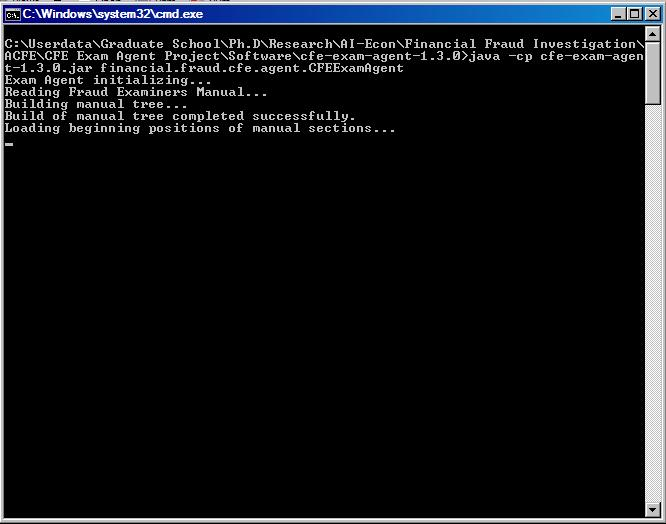
\includegraphics[scale=0.75]{screen_shot_1.jpg}
\caption{CFE Agent Startup}
\end{figure}


In Fig. 5, the screen shows the completion of the startup sequence of the CFE Agent.  First, the CFE Agent gives a line-by-line report showing the nodes loaded into the tree data structure.  Then, it shows some additional configuration information showing the exam file, execution mode, and runtime status.  At this point, the CFE Agent is ready to begin the exam.

\begin{figure}
\centering
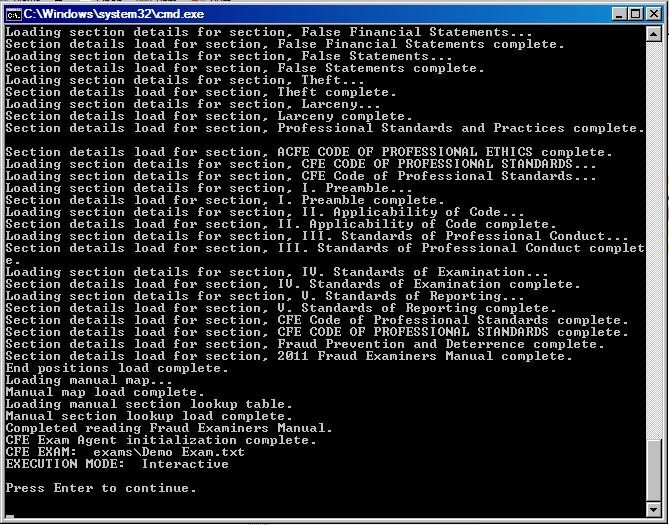
\includegraphics[scale=0.75]{screen_shot_2.jpg}
\caption{CFE Agent Startup Completed}
\end{figure}

In Fig. 6, the first question of the exam is shown along with four possible answers.  After the user presses return, the CFE Agent selects the optimal algorithm for that particular question and executes it.  

\begin{figure}
\centering
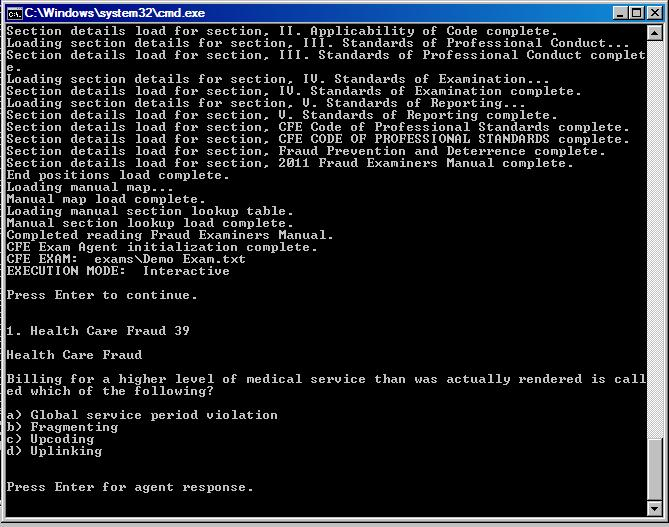
\includegraphics[scale=0.75]{screen_shot_3.jpg}
\caption{First Question}
\end{figure}

Fig. 7 shows log detail for the CFE Agent as it attempts to choose the correct answer for the first question.  First, as described in the discussion of the question profile, the agent makes an assignment to a question profile category based on some key features of the question, (whether it's a true-false question, a question at least one of whose options contains more than 4 words, etc.).  Once it assesses the question profile, it chooses an algorithm which based on prior experience exhibits maximum accuracy on questions having the same profile.  For this question, the profile assignment is category 2, meaning the question has been categorized as a ``definition'' question – essentially one which attempts to test for knowledge of domain-specific vocabulary.  The experience data of the Agent indicates the best performing algorithm is the Max Frequency algorithm, which when applied for this question results in the selection of choice c, the correct answer.

\begin{figure}
\centering
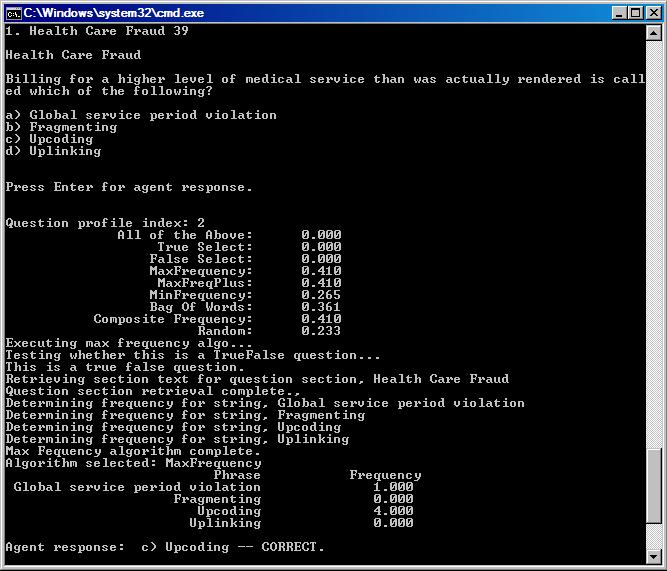
\includegraphics[scale=0.75]{screen_shot_4.jpg}
\caption{First Question Completed}
\end{figure}

Fig. 8 shows the CFE Agent answer the second question.  This question appears to be similar to the first in that it also earns a category assignment of 2, meaning it is another ``definition'' question.  By the same experience-based reasoning as in the first question, the agent applies the Max Frequency algorithm and selects answer a, the correct answer.

\begin{figure}
\centering
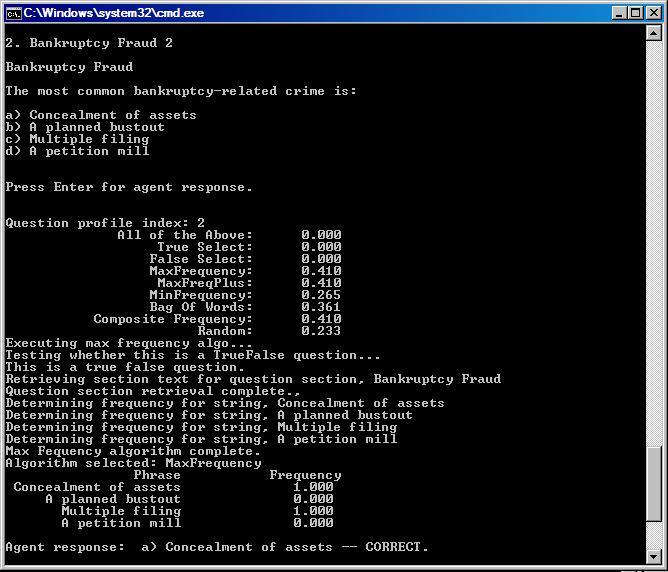
\includegraphics[scale=0.75]{screen_shot_5.jpg}
\caption{Second Question}
\end{figure}

Fig. 9 shows an attempt at the third question.  However, this time the agent is not successful at choosing the right answer.  Again, it assigns this question to the same category as the two prior questions and uses the same Max Frequency algorithm, but it is led astray by the fact that the fourth option, ``cost'' is a common word whose frequency in the section corpus is over-weighted relative to the other options for this question.  This is an example where the current level of sophistication of the agent is insufficient to correctly answer questions one of the options may consists of a word or phrase that might be over-represented in the corpus.  Further work will need to be done to develop the natural language processing algorithm to compensate for this over-weighting, while preserving its relative success on other questions in the same category.

\begin{figure}
\centering
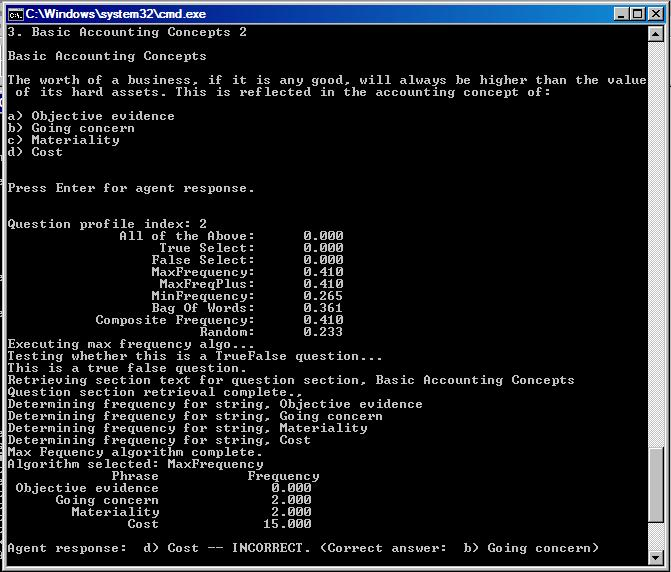
\includegraphics[scale=0.75]{screen_shot_6.jpg}
\caption{Third Question}
\end{figure}

Fig. 10 shows the final question, which is one of a different type --- an ``All of the Above'' question.  Here, the CFE Agent chooses an algorithm appropriately called ``All of the Above'' because it simply selects ``All of the Above'' whenever its an option.  (As shown in the data table, this algorithm has a remarkable 86\% success rate, lending one to question certain aspects of the CFE Exam’s design, as mentioned earlier.)  The agent applies this algorithm and gets the answer correct.  Finally, the agent terminates.

\begin{figure}
\centering
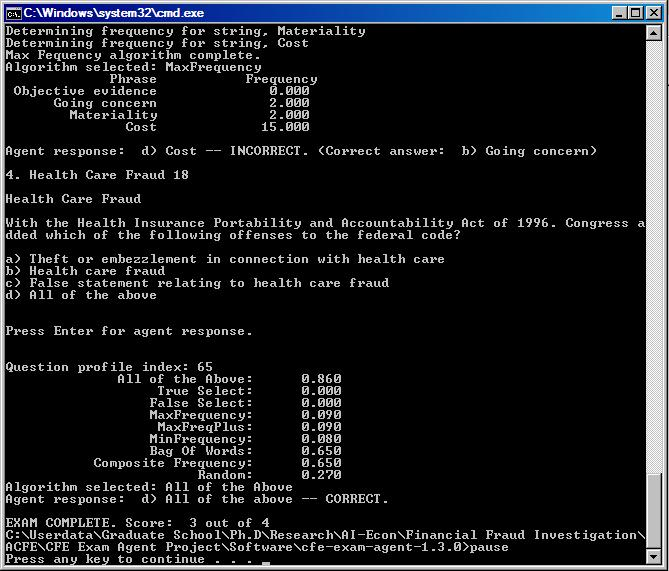
\includegraphics[scale=0.75]{screen_shot_7.jpg}
\caption{Final Question and Termination}
\end{figure}

